%==============================================================================
% Artigo 2 - FGA0261 Inteligência Artificial II - 2026.2
% Formato: IEEE conference (classe IEEEtran, máximo 4 páginas)
% Entrega: 09/10/2026, pelo Microsoft Teams
%
% CONVENÇÃO DESTE ARQUIVO: uma frase por linha.
% Isso não muda o PDF (o LaTeX junta as linhas) e mantém o git diff legível
% quando as duas pessoas da dupla editam o mesmo parágrafo.
%
% Compilar: make no Linux; .\build.ps1 no Windows sem Perl/latexmk.
%==============================================================================
\documentclass[conference]{IEEEtran}

\usepackage[T1]{fontenc}
\usepackage[utf8]{inputenc}
% Para hifenização correta em português, descomente a linha abaixo.
% Exige o pacote texlive-langportuguese no Arch.
% \usepackage[brazil]{babel}

\usepackage{cite}
\usepackage{amsmath,amssymb,amsfonts}
\usepackage{graphicx}
\usepackage{booktabs}
\usepackage{url}

\graphicspath{{figs/}}
\usepackage{multirow}

% Gerado por src/report.py a partir dos JSON de src/results/ e results-mean/.
% NÃO editar à mão: todo número do artigo sai daqui.
% Gerado por src/report.py — NÃO EDITAR À MÃO.
% Precisando de um número novo no texto, acrescente a macro ao report.py.

% --- agregação max ---
\newcommand{\ResultBestModelMax}{Autoencoder LSTM}
\newcommand{\ResultLimiarAucPrMax}{0,5009 $\pm$ 0,0066}
\newcommand{\ResultLimiarFMax}{0,316 $\pm$ 0,017}
\newcommand{\ResultLimiarPrecisionMax}{0,741 $\pm$ 0,021}
\newcommand{\ResultLimiarRecallMax}{0,201 $\pm$ 0,012}
\newcommand{\ResultLimiarParamsMax}{12}
\newcommand{\ResultLimiarSecondsMax}{0,1}
\newcommand{\ResultLimiarLatencyMax}{9,1}
\newcommand{\ResultLimiarPicoMax}{0,9021 $\pm$ 0,0119}
\newcommand{\ResultLimiarGanhoMax}{0,2448 $\pm$ 0,0322}
\newcommand{\ResultLimiarDerivaMax}{0,1098 $\pm$ 0,0036}
\newcommand{\ResultLimiarTravadoMax}{0,0519 $\pm$ 0,0025}
\newcommand{\ResultLimiarLacunaMax}{0,0449 $\pm$ 0,0040}
\newcommand{\ResultPcaAucPrMax}{0,4833 $\pm$ 0,0053}
\newcommand{\ResultPcaFMax}{0,372 $\pm$ 0,006}
\newcommand{\ResultPcaPrecisionMax}{0,801 $\pm$ 0,018}
\newcommand{\ResultPcaRecallMax}{0,242 $\pm$ 0,004}
\newcommand{\ResultPcaParamsMax}{6\,120}
\newcommand{\ResultPcaSecondsMax}{1,4}
\newcommand{\ResultPcaLatencyMax}{3,1}
\newcommand{\ResultPcaPicoMax}{0,9993 $\pm$ 0,0001}
\newcommand{\ResultPcaGanhoMax}{0,2028 $\pm$ 0,0183}
\newcommand{\ResultPcaDerivaMax}{0,0530 $\pm$ 0,0034}
\newcommand{\ResultPcaTravadoMax}{0,0601 $\pm$ 0,0087}
\newcommand{\ResultPcaLacunaMax}{0,0478 $\pm$ 0,0033}
\newcommand{\ResultAutoencoderAucPrMax}{0,5109 $\pm$ 0,0067}
\newcommand{\ResultAutoencoderFMax}{0,395 $\pm$ 0,010}
\newcommand{\ResultAutoencoderPrecisionMax}{0,776 $\pm$ 0,019}
\newcommand{\ResultAutoencoderRecallMax}{0,265 $\pm$ 0,008}
\newcommand{\ResultAutoencoderParamsMax}{12\,246}
\newcommand{\ResultAutoencoderSecondsMax}{197,5}
\newcommand{\ResultAutoencoderLatencyMax}{4,4}
\newcommand{\ResultAutoencoderPicoMax}{0,9619 $\pm$ 0,0081}
\newcommand{\ResultAutoencoderGanhoMax}{0,2697 $\pm$ 0,0127}
\newcommand{\ResultAutoencoderDerivaMax}{0,0874 $\pm$ 0,0195}
\newcommand{\ResultAutoencoderTravadoMax}{0,0679 $\pm$ 0,0184}
\newcommand{\ResultAutoencoderLacunaMax}{0,0461 $\pm$ 0,0047}

% --- agregação mean ---
\newcommand{\ResultBestModelMean}{Autoencoder LSTM}
\newcommand{\ResultLimiarAucPrMean}{0,3814 $\pm$ 0,0102}
\newcommand{\ResultLimiarFMean}{0,131 $\pm$ 0,016}
\newcommand{\ResultLimiarPrecisionMean}{0,513 $\pm$ 0,029}
\newcommand{\ResultLimiarRecallMean}{0,075 $\pm$ 0,010}
\newcommand{\ResultLimiarParamsMean}{12}
\newcommand{\ResultLimiarSecondsMean}{0,1}
\newcommand{\ResultLimiarLatencyMean}{10,6}
\newcommand{\ResultLimiarPicoMean}{0,0840 $\pm$ 0,0089}
\newcommand{\ResultLimiarGanhoMean}{0,4704 $\pm$ 0,0526}
\newcommand{\ResultLimiarDerivaMean}{0,1268 $\pm$ 0,0061}
\newcommand{\ResultLimiarTravadoMean}{0,0567 $\pm$ 0,0054}
\newcommand{\ResultLimiarLacunaMean}{0,0459 $\pm$ 0,0042}
\newcommand{\ResultPcaAucPrMean}{0,5067 $\pm$ 0,0094}
\newcommand{\ResultPcaFMean}{0,286 $\pm$ 0,022}
\newcommand{\ResultPcaPrecisionMean}{0,817 $\pm$ 0,013}
\newcommand{\ResultPcaRecallMean}{0,173 $\pm$ 0,016}
\newcommand{\ResultPcaParamsMean}{6\,120}
\newcommand{\ResultPcaSecondsMean}{1,2}
\newcommand{\ResultPcaLatencyMean}{8,5}
\newcommand{\ResultPcaPicoMean}{0,4916 $\pm$ 0,0220}
\newcommand{\ResultPcaGanhoMean}{0,7026 $\pm$ 0,0307}
\newcommand{\ResultPcaDerivaMean}{0,0670 $\pm$ 0,0065}
\newcommand{\ResultPcaTravadoMean}{0,0590 $\pm$ 0,0064}
\newcommand{\ResultPcaLacunaMean}{0,0489 $\pm$ 0,0053}
\newcommand{\ResultAutoencoderAucPrMean}{0,5634 $\pm$ 0,0172}
\newcommand{\ResultAutoencoderFMean}{0,309 $\pm$ 0,024}
\newcommand{\ResultAutoencoderPrecisionMean}{0,839 $\pm$ 0,040}
\newcommand{\ResultAutoencoderRecallMean}{0,189 $\pm$ 0,016}
\newcommand{\ResultAutoencoderParamsMean}{12\,246}
\newcommand{\ResultAutoencoderSecondsMean}{188,4}
\newcommand{\ResultAutoencoderLatencyMean}{6,6}
\newcommand{\ResultAutoencoderPicoMean}{0,3012 $\pm$ 0,0058}
\newcommand{\ResultAutoencoderGanhoMean}{0,6969 $\pm$ 0,0356}
\newcommand{\ResultAutoencoderDerivaMean}{0,3511 $\pm$ 0,0669}
\newcommand{\ResultAutoencoderTravadoMean}{0,0604 $\pm$ 0,0069}
\newcommand{\ResultAutoencoderLacunaMean}{0,0473 $\pm$ 0,0066}

% --- tabela principal, inserida no texto por \ResultTable ---
\newcommand{\ResultTable}{%
\begin{table}[htbp]
\caption{Desempenho no conjunto de teste sob as duas regras de agregação do escore de janela (média $\pm$ desvio padrão de três execuções). A agregação inverte o veredito: sob o máximo os três detectores praticamente empatam, enquanto sob a média o autoencoder se separa.}
\label{tab:resultados}
\centering
\begin{tabular}{llcr}
\toprule
\textbf{Agregação} & \textbf{Modelo} & \textbf{AUC-PR} & \textbf{Parâm.} \\
\midrule
\multirow{3}{*}{Máximo} & Limiar 3$\sigma$ & 0,5009 $\pm$ 0,0066 & 12 \\
 & PCA & 0,4833 $\pm$ 0,0053 & 6\,120 \\
 & \textbf{Autoencoder LSTM} & \textbf{0,5109 $\pm$ 0,0067} & 12\,246 \\
\midrule
\multirow{3}{*}{Média} & Limiar 3$\sigma$ & 0,3814 $\pm$ 0,0102 & 12 \\
 & PCA & 0,5067 $\pm$ 0,0094 & 6\,120 \\
 & \textbf{Autoencoder LSTM} & \textbf{0,5634 $\pm$ 0,0172} & 12\,246 \\
\bottomrule
\end{tabular}
\end{table}
}


\begin{document}

\title{Detecção Não Supervisionada de Falhas de Sensor em Telemetria Veicular com Autoencoder Recorrente}

\author{
\IEEEauthorblockN{Gustavo Xavier Evangelista}
\IEEEauthorblockA{\textit{FCTE - Faculdade de Ciências e Tecnologias em Engenharia} \\
\textit{Universidade de Brasília} \\
Brasília, Brasil \\
Matrícula: 241025247 \\
241025247@aluno.unb.br}
\and
\IEEEauthorblockN{Heitor Macêdo Ricardo}
\IEEEauthorblockA{\textit{FCTE - Faculdade de Ciências e Tecnologias em Engenharia} \\
\textit{Universidade de Brasília} \\
Brasília, Brasil \\
Matrícula: 241039073 \\
241039073@aluno.unb.br}
}

\maketitle

\begin{abstract}
% 150-200 palavras, JÁ COM O NÚMERO PRINCIPAL DO RESULTADO.
% Escrever por último, depois que a tabela estiver fechada.
% Estrutura: contexto -> lacuna -> o que foi feito -> número principal -> implicação.
\end{abstract}

\begin{IEEEkeywords}
% 4 a 6 termos separados por vírgula.
\end{IEEEkeywords}

%==============================================================================
\section{Introdução}
%==============================================================================

A telemetria veicular embarcada consiste na aquisição e no registro contínuos de variáveis do veículo, como rotação, velocidade, temperaturas, pressões e atuação do acelerador \cite{weber2023automotive,kang2016intrusion}.
Essas variáveis podem ser obtidas pelo sistema de diagnóstico de bordo de segunda geração (On-Board Diagnostics II, OBD-II) ou circular entre unidades de controle eletrônico (Electronic Control Units, ECUs) pela rede de área de controladores (Controller Area Network, CAN) \cite{weber2023automotive,kang2016intrusion}.
Como os sinais descrevem o estado físico usado para supervisão e controle, falhas de sensor podem comprometer tanto a confiabilidade do histórico quanto decisões de manutenção e segurança \cite{isermann2005model,kang2016intrusion}.

Uma salvaguarda elementar consiste em aceitar cada leitura somente quando ela pertence a uma faixa física predefinida, procedimento de baixo custo associado à verificação clássica de limites \cite{isermann2005model}.
Essa regra detecta valores impossíveis, mas não identifica uma falha cuja saída permaneça plausível enquanto perde a relação com os demais sinais \cite{isermann2005model,chandola2009anomaly}.
Considere-se uma falha de ganho, isto é, uma calibração multiplicativa incorreta: se o programa embarcado (firmware) trocar a constante \texttt{RPM\_ESCALA} de 0,25 para 0,125, a interface de programação de aplicações (API) passa a registrar o dobro das rotações por minuto (RPM) reais \cite{evangelista2026sensorfaults}.
Nesse cenário, 3.000 RPM reais tornam-se 6.000 RPM registrados, valor que continua válido e, portanto, atravessa a verificação de faixa sem alerta \cite{evangelista2026sensorfaults}.
Surge, assim, a lacuna entre validar cada canal isoladamente e detectar incoerências temporais e multivariadas, isto é, entre múltiplos canais, dentro do domínio admissível \cite{chandola2009anomaly,malhotra2016lstm}.

Em telemetria veicular multivariada de baixa taxa, quanto um autoencoder recorrente treinado apenas em operação normal supera detectores estatísticos e lineares na identificação de falhas de sensor injetadas, e a que custo computacional?

Este trabalho compara um limiar de três desvios-padrão ($3\sigma$), a análise de componentes principais (Principal Component Analysis, PCA) e um autoencoder recorrente, rede neural treinada para reconstruir suas entradas e implementada com memória de longo e curto prazo (Long Short-Term Memory, LSTM), sob o mesmo protocolo de falhas injetadas em telemetria OBD-II e com avaliação de desempenho e custo computacional \cite{lakhina2004diagnosing,malhotra2016lstm,weber2023automotive}.

%==============================================================================
\section{Trabalhos Relacionados}
%==============================================================================

Entre as abordagens por limiar e métodos estatísticos, Chandola, Banerjee e Kumar organizam detectores segundo as hipóteses usadas para separar o comportamento normal do anômalo, mostrando que regras simples dependem de uma definição adequada de normalidade \cite{chandola2009anomaly}.
Para dados multivariados, Lakhina, Crovella e Diot empregam PCA para decompor medições em subespaços normal e anômalo, de modo que o resíduo em relação à estrutura linear aprendida produza uma medida de desvio denominada escore de anomalia \cite{lakhina2004diagnosing}.
Essas estratégias oferecem referências interpretáveis e de baixo custo, porém uma faixa por canal ignora dependências entre sinais e a PCA se restringe a relações lineares \cite{chandola2009anomaly,lakhina2004diagnosing}.

Nos métodos baseados em reconstrução de séries temporais, Malhotra et al. propõem um codificador-decodificador LSTM treinado em sequências normais e usam o erro de reconstrução para sinalizar observações incompatíveis com o padrão aprendido \cite{malhotra2016lstm}.
O método de detecção não supervisionada de anomalias (UnSupervised Anomaly Detection, USAD) combina dois autoencoders que se refinam competitivamente para detectar anomalias em séries temporais multivariadas com baixa sobrecarga de inferência \cite{audibert2020usad}.
Já o OmniAnomaly combina recorrência com uma representação probabilística interna para modelar dependências temporais e incerteza em sinais multivariados \cite{su2019robust}.
Em conjunto, esses trabalhos motivam modelos não supervisionados capazes de aprender relações não lineares sem exigir exemplos rotulados de cada falha \cite{malhotra2016lstm,audibert2020usad,su2019robust}.

No domínio veicular, Taylor, Leblanc e Japkowicz treinam uma LSTM para prever a próxima palavra de dados no CAN e sinalizar ataques sintéticos pela improbabilidade dos bits observados \cite{taylor2016automobile}.
Kang e Kang classificam pacotes CAN normais e maliciosos com uma rede neural profunda treinada sobre atributos probabilísticos, abordagem supervisionada na qual exemplos das duas classes são fornecidos durante o ajuste \cite{kang2016intrusion}.
Em outra frente, o Automotive OBD-II Dataset disponibiliza dez sinais físicos coletados em condução real, mas não fornece um catálogo rotulado de falhas de sensores para treinamento supervisionado \cite{weber2023automotive}.

O diferencial deste artigo está em avaliar falhas de sensor, e não ataques ao tráfego CAN, mediante a comparação controlada de um limiar, um modelo linear e um autoencoder recorrente sobre a mesma telemetria OBD-II de baixa taxa, incluindo a falha de ganho que permanece dentro da faixa válida e registrando também o custo computacional \cite{chandola2009anomaly,lakhina2004diagnosing,malhotra2016lstm,taylor2016automobile,kang2016intrusion,weber2023automotive}.

%==============================================================================
\section{Metodologia}
%==============================================================================

\subsection{Conjunto de dados}

Foi utilizado o Automotive OBD-II Dataset \cite{weber2023automotive}, distribuído publicamente sob licença CC BY 4.0.
A coleção reúne 81 sessões de condução de um mesmo veículo, registradas entre 2017 e 2018 pela porta de diagnóstico de bordo (OBD-II), somando 70,0 horas de operação.
Cada sessão registra dez grandezas, entre as quais rotação do motor, velocidade, fluxo de ar admitido, pressão absoluta no coletor e duas leituras redundantes do pedal do acelerador.

Quatro sessões cujo nome indica condição atípica de condução ou erro de medição foram removidas, restando 77: o detector é treinado apenas em operação normal, e essas sessões não oferecem garantia de o serem.

\subsection{Representação canônica e reamostragem}

As linhas do arquivo chegam a uma taxa nominal de 11,3\,Hz, mas essa taxa é aparente: cada linha repete o último valor conhecido de cada canal.
A taxa real de atualização foi medida contando quantas vezes o valor efetivamente muda, e o canal mais rápido chega a 1,11\,Hz.
Por esse motivo os sinais foram reamostrados para 1\,Hz, retendo o último valor válido de cada segundo.
Reamostrar na taxa nominal faria o modelo de reconstrução aprender a copiar valores retidos, produzindo erro artificialmente baixo e desempenho inflado.

Seis canais foram mantidos, por apresentarem taxa real de mudança superior a 0,3\,Hz e não serem redundantes entre si: rotação, velocidade, fluxo de ar, pressão no coletor, temperatura do ar admitido e posição do pedal.
As duas leituras do pedal apresentam correlação de 0,99 entre si, por constituírem o par redundante do projeto de segurança do veículo, e apenas uma foi preservada.
Os três canais restantes mudam a menos de 0,04\,Hz e foram descartados.

\subsection{Segmentação e janelamento}

Cada sessão foi dividida nos intervalos superiores a 2\,s sem amostra, e cada trecho contínuo passou a constituir um segmento independente.
Intervalos longos são esperados em telemetria embarcada: sem conectividade, os quadros são acumulados em memória e transmitidos ao reestabelecer o enlace, e o maior observado foi de 603,9\,s.
Trata-se de operação normal, de modo que um intervalo não pode atravessar uma janela sob pena de o detector aprender a sinalizar todo retorno à cobertura.

Os segmentos foram recortados em janelas deslizantes de 60\,s com passo de 10\,s, descartando-se os 19 segmentos menores que uma janela.
O procedimento produziu 85 segmentos contínuos e 23\,073 janelas, cada uma um tensor de 60 amostras por 6 canais.

\subsection{Divisão e normalização}

A divisão em treino, validação e teste foi feita \emph{por sessão}, nunca por janela.
Janelas vizinhas compartilham 50 das 60 amostras, e um sorteio por janela colocaria trechos quase idênticos nos dois lados da avaliação.
O sorteio das sessões usa semente própria e fixa, independente das sementes de treinamento, para que a variação entre execuções meça variação de treinamento e não troca das sessões avaliadas.

A divisão resultou em 17\,229 janelas de treino (54 sessões), 2\,653 de validação (12 sessões) e 3\,191 de teste (11 sessões).
As proporções por janela afastam-se das frações nominais de 70\,\%, 15\,\% e 15\,\% porque as sessões têm durações distintas, entre 12,2 e 134,7 minutos.
A média e o desvio padrão de cada canal foram calculados exclusivamente sobre o treino e aplicados aos três conjuntos, evitando vazamento das estatísticas de avaliação para o ajuste.

\subsection{Protocolo de injeção de falhas}

Como o detector é treinado sem rótulos de falha, as anomalias do conjunto de avaliação foram injetadas de forma controlada em janelas normais, o que torna conhecida a posição exata de cada falha.
As cinco classes correspondem a modos de falha documentados em telemetria veicular embarcada, e não a perturbações arbitrárias.

A \emph{falha de ganho} multiplica um canal por um fator constante, reproduzindo a troca de uma constante de escala no firmware sem atualização correspondente no servidor.
O \emph{sensor travado} congela a leitura no último valor.
A \emph{deriva} soma um viés que cresce linearmente até três desvios padrão do canal, reproduzindo deriva térmica.
O \emph{pico} soma seis desvios padrão em três instantes isolados, reproduzindo ruído elétrico no barramento.
A \emph{lacuna} repete o último valor por 3 a 8\,s, reproduzindo perda curta de pacotes.

As injeções operam sobre as grandezas físicas, antes da normalização, pois um erro de escala só é interpretável na unidade original.
Cada falha começa em um instante sorteado dentro da primeira metade da janela, garantindo trecho afetado suficiente para a medida de latência.
Vinte por cento das janelas de validação e teste foram corrompidas, com as cinco classes em rodízio; o treino permanece íntegro.

Aplicando-se limites de plausibilidade física a cada canal, nenhuma das 3\,191 janelas normais de teste é sinalizada, mas as falhas de ganho, sensor travado e lacuna atravessam a verificação em 100\,\% dos casos, contra 32,5\,\% de detecção para a deriva e 96,2\,\% para o pico.
Três das cinco classes são invisíveis a uma regra de faixa, o que delimita o que um detector aprendido precisa acrescentar.

\subsection{Modelos avaliados}

Os três detectores compartilham a mesma interface e o mesmo protocolo: são ajustados somente em janelas normais de treino, produzem um escore por amostra e agregam esse escore pelo máximo ao longo da janela.
A agregação única é necessária para que a comparação meça o mecanismo de pontuação, e não a forma de resumir a janela.

O \emph{limiar} constitui a linha de base não aprendida.
Para cada canal, estima média e desvio padrão na operação normal e atribui a cada amostra o maior afastamento padronizado entre os canais, reproduzindo a verificação que seria escrita diretamente no firmware.

A \emph{análise de componentes principais} (PCA) atua como autoencoder linear: projeta a janela em subespaço de menor dimensão, reconstrói e usa o erro de reconstrução como escore, respondendo se a não linearidade é necessária ao problema.

O \emph{autoencoder recorrente} comprime a janela por uma rede de memória de longo e curto prazo (LSTM) \cite{hochreiter1997lstm} e a reconstrói a partir da representação latente \cite{goodfellow2016deep}.
Por processar a janela como sequência, dispõe da dependência temporal que os dois primeiros ignoram.
A dimensão latente é idêntica à do PCA, de modo que a diferença observada entre ambos seja atribuível à não linearidade e à memória, e não à capacidade de compressão.

No PCA e no autoencoder, a dimensão latente foi fixada em 16.
O codificador recorrente possui uma camada LSTM com 32 unidades seguida de projeção linear para o gargalo, enquanto o decodificador recebe esse vetor repetido pelos 60 instantes, emprega outra camada LSTM com 32 unidades e projeta a saída para os seis canais.
O ajuste minimizou o erro quadrático médio com AdamW, taxa de aprendizado de $10^{-3}$, decaimento de pesos de $10^{-4}$ e lotes de 64 janelas, por no máximo 30 épocas.
O treinamento foi interrompido após cinco épocas sem redução mínima de $10^{-4}$ na perda da validação normal, restaurando-se os parâmetros da melhor época.

\subsection{Calibração e métricas}

O limiar de decisão de cada detector é calibrado sobre a distribuição de escores das janelas normais de validação, nunca sobre o teste, que é consultado uma única vez ao final.

A métrica principal é a área sob a curva de precisão e revocação (AUC-PR).
A escolha decorre do desequilíbrio entre as classes: janelas anômalas constituem 20\,\% do conjunto de avaliação, e nesse regime a acurácia é inexpressiva, pois um detector que classifique tudo como normal já alcança 80\,\%.
A área sob a curva ROC também é inadequada, porque o grande número de verdadeiros negativos mantém a taxa de falso positivo baixa mesmo quando a precisão é ruim \cite{saito2015precision}; a AUC-PR, por depender da precisão, não apresenta essa complacência.

São reportadas ainda a medida F1, a precisão e a revocação no limiar calibrado, bem como o número de parâmetros aprendidos.
Acrescenta-se a \emph{latência de detecção}, definida como o número de amostras entre o início da falha e o instante em que o escore cruza o limiar.
A latência é relevante porque um detector que sinalize a falha tarde demais não cumpre a função de alarme, ainda que sua AUC-PR seja alta.

Os resultados foram obtidos com três sementes, e são reportados como média e desvio padrão entre as execuções.

%==============================================================================
\section{Resultados}
%==============================================================================
% Orçamento: ~0,8 página. Os números vêm de src/results/ via report.py.
% NENHUM valor pode ser digitado aqui: cite a macro.

\ResultTable

\begin{figure}[htbp]
\centering
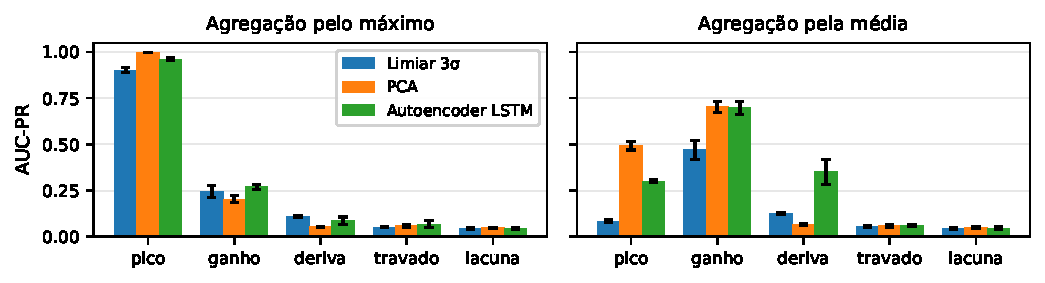
\includegraphics[width=\columnwidth]{auc-pr-por-classe.pdf}
\caption{AUC-PR por classe de falha sob as duas regras de agregação.
A ordenação entre os detectores se inverte conforme a regra: o máximo privilegia a falha pontual e a média, a sustentada.}
\label{fig:auc-por-classe}
\end{figure}

% A TEXTO (#38): comentar o que a Tabela~\ref{tab:resultados} e a
% Figura~\ref{fig:auc-por-classe} NÃO mostram, sem recitar números.

%==============================================================================
\section{Discussão e Limitações}
%==============================================================================

\subsection{A regra de agregação decide o veredito}

O resultado mais informativo do experimento não está em qual detector vence, e sim em quanto a resposta depende de uma decisão de protocolo aparentemente secundária.
Sob agregação pelo máximo os três detectores ficam a menos de três centésimos de distância em AUC-PR, e a tabela converge para um referendo sobre a classe pico.
Sob agregação pela média o autoencoder passa a \ResultAutoencoderAucPrMean{} contra \ResultLimiarAucPrMean{} da linha de base, uma diferença de quase cinquenta por cento.

Tomar o máximo faz o escore depender de um único instante, privilegiando a falha pontual e descartando a informação de que a degradação persiste; tomar a média dilui o pico isolado entre sessenta amostras e acumula o desvio sustentado.
Nenhuma das duas é correta em absoluto, pois medem fenômenos diferentes, e a escolha precede qualquer comparação entre modelos.

\subsection{Onde o autoencoder se separa}

A vantagem do autoencoder recorrente concentra-se na deriva, com \ResultAutoencoderDerivaMean{} sob agregação pela média contra \ResultPcaDerivaMean{} do PCA.
Como ambos comprimem para a mesma dimensão latente, a diferença decorre da não linearidade e da leitura sequencial, e não da capacidade de compressão: a deriva é o modo de falha cuja assinatura existe apenas na evolução temporal, pois nenhum instante isolado é anômalo.

O comportamento oposto aparece no pico, onde o PCA alcança \ResultPcaPicoMax{} sob agregação pelo máximo e supera o autoencoder.
Uma projeção linear reconstrói mal um valor extremo isolado, enquanto a rede recorrente acomoda parcialmente a perturbação e reduz o próprio erro: a capacidade que beneficia a deriva prejudica o pico.

\subsection{O que o experimento não resolve}

As classes sensor travado e lacuna permanecem próximas do acaso nos três detectores e nas duas agregações.
Ambas foram injetadas em sinais que atravessam longos trechos genuinamente constantes em operação normal, como a velocidade com o veículo parado; congelar um sinal já congelado não produz assinatura detectável, de modo que o resultado mede a inadequação do par falha--canal, e não a incapacidade dos modelos.

A progressão entre as três estratégias é, ainda assim, consistente: a validação de faixa não sinaliza nenhuma janela com ganho, sensor travado ou lacuna, a linha de base estatística recupera parte do ganho, e o detector aprendido acrescenta a deriva.
Cada nível incorpora o que o anterior descartava: o valor isolado, depois sua distribuição, por fim a relação temporal entre canais.

\subsection{Limitações}

As anomalias avaliadas são \emph{injetadas}, não observadas: o protocolo controla posição e severidade, o que permite medir latência e desempenho por classe, mas não garante que falhas reais apresentem a mesma assinatura.
Os dados provêm de um único veículo e não contêm os canais do protótipo de competição que motivou o trabalho, de modo que a validade externa restringe-se a telemetria de arquitetura semelhante.
A reamostragem para 1\,Hz descarta dinâmica rápida que um barramento dedicado registraria.

O autoencoder não convergiu dentro do orçamento de trinta épocas: a melhor época situou-se entre a vigésima oitava e a trigésima em todas as execuções e a parada antecipada nunca foi acionada, de modo que os valores reportados constituem um limite inferior dessa arquitetura.
As três execuções por configuração sustentam estimativa de dispersão, não teste de significância.

%==============================================================================
\section{Conclusão}
%==============================================================================
% Orçamento: ~0,2 página. De 3 a 4 frases, respondendo a pergunta da Introdução.
% Nenhum resultado novo aqui.

%==============================================================================
\bibliographystyle{IEEEtran}
\bibliography{refs}

\end{document}
